%%%%%%%%%%%%%%%%%%%%%%%%%%%%%%%%%%%%%%%%%
% Journal Article
% LaTeX Template
% Version 1.3 (9/9/13)
%
% This template has been downloaded from:
% http://www.LaTeXTemplates.com
%
% Original author:
% Frits Wenneker (http://www.howtotex.com)
%
% License:
% CC BY-NC-SA 3.0 (http://creativecommons.org/licenses/by-nc-sa/3.0/)
%
%%%%%%%%%%%%%%%%%%%%%%%%%%%%%%%%%%%%%%%%%

%----------------------------------------------------------------------------------------
%	PACKAGES AND OTHER DOCUMENT CONFIGURATIONS
%----------------------------------------------------------------------------------------

\documentclass[twoside]{article}

\usepackage{mathtools}
\newcommand\numberthis{\addtocounter{equation}{1}\tag{\theequation}}
% row color
\usepackage{color, colortbl}
\definecolor{Gray}{gray}{0.95}

\usepackage{program}
\usepackage{graphicx}

\usepackage[sc]{mathpazo} % Use the Palatino font
\usepackage[T1]{fontenc} % Use 8-bit encoding that has 256 glyphs
\linespread{1.05} % Line spacing - Palatino needs more space between lines
\usepackage{microtype} % Slightly tweak font spacing for aesthetics

\usepackage[hmarginratio=1:1,top=32mm,columnsep=20pt]{geometry} % Document margins
\usepackage{multicol} % Used for the two-column layout of the document
\usepackage[hang, small,labelfont=bf,up,textfont=it,up]{caption} % Custom captions under/above floats in tables or figures
\usepackage{booktabs} % Horizontal rules in tables
\usepackage{float} % Required for tables and figures in the multi-column environment - they need to be placed in specific locations with the [H] (e.g. \begin{table}[H])
\usepackage{hyperref} % For hyperlinks in the PDF

\usepackage{lettrine} % The lettrine is the first enlarged letter at the beginning of the text
\usepackage{paralist} % Used for the compactitem environment which makes bullet points with less space between them

\usepackage{abstract} % Allows abstract customization
\renewcommand{\abstractnamefont}{\normalfont\bfseries} % Set the "Abstract" text to bold
\renewcommand{\abstracttextfont}{\normalfont\small\itshape} % Set the abstract itself to small italic text

\usepackage{titlesec} % Allows customization of titles
\renewcommand\thesection{\Roman{section}} % Roman numerals for the sections
\renewcommand\thesubsection{\Roman{subsection}} % Roman numerals for subsections
\renewcommand\thesubsubsection{\Roman{subsubsection}} % Roman numerals for subsections

\titleformat{\section}[block]{\large\scshape\centering}{\thesection.}{1em}{} % Change the look of the section titles
\titleformat{\subsection}[block]{\large}{\thesubsection.}{1em}{} % Change the look of the section titles

\usepackage{fancyhdr} % Headers and footers
\pagestyle{fancy} % All pages have headers and footers
\fancyhead{} % Blank out the default header
\fancyfoot{} % Blank out the default footer
\fancyhead[C]{Metodi ed algoritmi di ottimizzazione per il problem solving $\bullet$ a.a. 2015/2016} % Custom header text
\fancyfoot[RO,LE]{\thepage} % Custom footer text

%----------------------------------------------------------------------------------------
%	TITLE SECTION
%----------------------------------------------------------------------------------------

\title{\vspace{-15mm}\fontsize{24pt}{10pt}\selectfont\textbf{A semi-parallel Tabu Search Heuristic Algorithm for Vehicle Routing Problem}} % Article title

\author{
\large
\textsc{Edoardo Rosa}\\[2mm] % Your name
\normalsize University of Bologna \\ % Your institution
\normalsize \href{mailto:edoardo.rosa@studio.unibo.it}{edoardo.rosa@studio.unibo.it} % Your email address
\vspace{-5mm}
}
\date{}

%----------------------------------------------------------------------------------------

\begin{document}

\maketitle % Insert title

\thispagestyle{fancy} % All pages have headers and footers

%----------------------------------------------------------------------------------------
%	ABSTRACT
%----------------------------------------------------------------------------------------

\begin{abstract}

\noindent % Dummy abstract text
This paper presents a tabu search heuristic for the standard vehicle routing problem with capacity and time restrictions. The algorithm use some parallel routines to improve speed and execution time remaining easy to use and understanding.
The results are presented running standard problems from the \url{http://www.coin-or.org/} library for VRP.
\noindent\newline
The code is available at \url{https://github.com/edoz90/VRP-tabu}.
\end{abstract}

%----------------------------------------------------------------------------------------
%	ARTICLE CONTENTS
%----------------------------------------------------------------------------------------

\begin{multicols}{2} % Two-column layout throughout the main article text

\section{Introduction}

\lettrine[nindent=0em,lines=3]{T}he vehicle routing problem (\emph{VRP}) is a combinatorial optimization and integer programming problem which asks "What is the optimal set of routes for a fleet of vehicles to traverse in order to deliver to a given set of customers?". It generalises the travelling salesman problem (TSP).

Determining the optimal solution is an \textit{NP-hard} problem in combinatorial optimization, so the size of problems that can be solved optimally is limited. The commercial solvers therefore tend to use heuristics due to the size of real world VRPs and the frequency that they may have to be solved. In this case we use a \emph{Tabu Search} algorithm.\newline
The VRP is defined on a complete graph $G=(V,E)$, where $V=\{v_{0}, v_{1},...,v_{n}\}$ is the vertexes set and $E=\{(v_{i},v{j}):\; v_{i},v{j}\in V\;, i\neq j\}$ is the edges set. Vertex $v_{0}$ is the depot at which $m$ identical vehicles are based, and the remaining vertexes represent the customers to be served. Each customer/vertex \textit{$i$} has a non-negative demand $q_{i}$ and a non negative service duration $\delta_{i}$. Each vehicle has a capacity $Q$ and the duration of its route cannot exceed $L$ time.

With each edge $(v_{i},v_{j})$ is associated a non-negative cost $c_{i,j}$ proportional to the travel time from vertex $i$ to $j$.
In this case the working time for each vehicle and the service duration are optional parameters.

The VRP consists of designing a set of least cost vehicle routes in such a way that:
\begin{itemize}
	\item every route start and ends at the depot;
	\item every city of $V\setminus\{v_{0}\}$ is visited exactly once by exactly one vehicle;
	\item the total demand of any vehicle route may not exceed $Q$;
	\item the total lenght of any route (travel plus service times) may not exceed $L$.
\end{itemize}

%------------------------------------------------
\clearpage
\section{Formulation}
$x_{ij}=1$ if the route goes from customer $i$ to customer $j$; $x_{ij}=0$ otherwise.\\
$z^{k}_{i}=1$ if the customer $i$ is visited by vehicle $k$.

\begin{equation*}
	VRP
	\begin{cases}
		\displaystyle Min\ \sum_{i=1}^{n}\sum_{j=1}^{n}c_{i,j}x_{i,j} \\
		\ \ \ \ \ \ \ \ \displaystyle\sum_{i=1}^{n}z^{k}_{i}=1,\ k=1,\dots,m \\
		\ \ \ \ \ \ \ \ \displaystyle\sum_{i=1}^{n}\sum_{j=1}^{n}q_{i}x_{ij} \le Q \\
		\ \ \ \ \ \ \ \ \displaystyle\sum_{i=1}^{n}\sum_{j=1}^{n}\delta_{i}x_{ij} \le L \\
		\ \ \ \ \ \ \ \ \displaystyle\sum_{i \in S} \sum_{j \notin S}x_{ij} \ge 1\;for\;S \subset V,\; S\ne \emptyset \\
		\ \ \ \ \ \ \ \ \ \ \ \ \ \ \ \ \ \ x_{ij} \in \{0,1\}
	\end{cases}
\end{equation*}
An alternative for the \textit{cut-set} constraint is:
\begin{equation*}
	\displaystyle\sum_{i\in S}\sum_{j\in S}x_{ij}\le \lvert S\rvert-1,\ \; \forall S\subset N,\ 2\le\lvert S\rvert\le n-1
\end{equation*}
The solution is a set $S=\{R_{1},R_{2},...,R_{m}\}$ of $m$ routes and each route is a set $R_{i}=\{v_{0},v_{r1},v_{r2},...v_{v0}\}$, feasible with respect to capacity and time constraints, and each vertex belongs to exactly one route.

The optimal solution $S^{*}$ is the one which is feasible and minimize the total cost of routes.
The sum of costs for each move from customer $i$ to $j$, denoted with $c_{i.j}$, is the cost of a single route; the sum of costs for all routes is the total cost of the solution.\\
The fitness function is:
\begin{equation}
F(S^{*}) = \sum_{r\in R} \sum_{(v_{i},v_{j})} c_{i,j} \label{eq:objfun}
\end{equation}
	
%------------------------------------------------

\section{Algorithm}
The algorithm creates and considers only feasible solutions; the assessment is based on the total cost of routes (\ref{eq:objfun}): no parameters for vehicle capacity or route duration excesses.\newline
The algorithm first creates an initial solution that is improved by a \textit{tabu search heuristic}; after each round of tabu search iterations the routes are refined.
\begin{program}
	\mbox{Algorithm}
	\BEGIN \\ %
	|routes| \gets InitialSolution()
	\WHILE \NOT stopCondition \DO
		|tabuSolution| \gets TabuSearch(|routes|);
		RefineAndOpt(|tabuSolution|);
		\IF f(|tabuSolution|) > f(|bestSolution|)
		\THEN
			|bestSolution| \gets |tabuSolution|
		\FI
		routes = |tabuSolution|;
	\OD
	print(|bestSolution|);
	\END
\end{program}

\subsection{Construction of an initial solution}
The construction of the initial solution $S'$ is based on an Iterated Local Search algorithm.

\begin{program}
	\mbox{Initial Solution:}
	\BEGIN \\ %
		|routes| \gets []
		\WHILE \NOT allCustomerServed \DO
			|route|.Add(|v0|); \rcomment{start from depot}
			|from| \gets |v0|;
			\WHILE routeIsFeasible \DO
				|to| \gets GetFreeNearest(|from|);
				\IF (|route|.Move(|from|, |to|)) 
				\THEN 
				|route|.Add(|to|); \rcomment{serve '|to|'}
				\ELSE
				|route|.Add(|v0|); \rcomment{close route}
				\EXIT;
				\FI
			\OD
			|routes|.Add(|route|); \rcomment{add route to solution}
		\OD
	\END
\end{program}
All routes are first initialized with the depot vertex. 

The customer closer to the depot is added as first move of first route; the next step is to find the customer closer to the already added customer and add it to the route.

This steps are repeated until the insertion of a customer would lead to capacity or working time violation.

When a route is closed, a new one is initialized and, again, the customer closer to the depot, not already served, is added to the route, and so on with all the customers.

If the number of routes is greater than $m$ or a customer can not be served, due to violation of constraints, the program stops.

The solution thus created is feasible and better than a solution produced from a random generation of moves.

\subsection{Tabu Search}
The tabu search heuristic starts from the current ILS solution $S^{'}$ and moves, at each iteration, to the best non-tabu solution in the neighbourhood. To ensure a broad exploration of the search space diversification, intensification and perturbation are used.

\textit{Intensification} is provided through a route refinement step that is applied periodically.\newline
All solutions created in tabu search iterations are feasible.\newline
Tabu search algorithm runs, for each customers in the routes, an ILS algorithm to find a better solution.

The routine for initial solution creates routes, specially the last, that do not form an optimal solution.

This heuristic tries to move customers from a route to another, in order to achieve a better solution, improving the total cost. 

Better solutions leads to routes that serve customers in their neighbourhood. For each customers $i$, the algorithm tries to insert, sequentially, all possible customers in the neighbourhood of $i$. The shift is performed only if the feasible solution created is better and the move is not tabu.\newline
The tabu search heuristic stops after the best solution $S*$ has failed to improve for a long time.

\subsubsection{Tabu list and aspiration criteria}
The tabu search algorithm is based on a \textit{tabu list} that contains all moves done during the routine. 

With each solution $s \in S$ is associated a set $B(s)$ of attributes $(i,k)$ if customer $i$ is visited by vehicle $k$. The neighbourhood $N(s)$ of a solution $s$ is defined by applying a simple operator that removes an attribute $(i,k)$ from $B(s)$ and replaces it with an attribute $(i,k')$, where $k\neq k'$. 

The operation within attributes represents a \textit{move} and all moves are stored in a tabu list to ensure to avoid local minimum and cycling.\newline
When a move is performed, the attribute is considered tabu for $\tau$ iterations and, any move adding at least one of these attributes, cannot be performed unless it satisfies the aspiration criteria.
The tabu list tenure $\tau$ is fixed at $n*0.7$, where $n$ is the number of customers.\newline
The aspiration criteria overrides the tabu status of a move if this yields a solution $s$ such that $f(s)$ is smaller than the cost of best solution found so far.\newline
To overcome local minimum the size of tabu list is not fixed but vary in the interval $[7, 15]$. The size is increased when the solution found at end is not better, decreased otherwise.

\subsubsection{Diversification}
An iteration of tabu search algorithm can bring to a non-best solution which could mean that a local minimum is reached or the algorithm is cycling to same solutions; to avoid this behaviour if no improvements are made, the solution is degraded.

To degrade a solution the algorithm saves a list of non-best solutions and the worst is chosen to substitute the actual one.\newline
In addition, to diversify the search, a penalty term is added to any solution $\hat{s}$ such that $f(\hat{s}) \ge f(s)$. The factor is proportional to the addition frequency of its attributes and a scaling factor $\lambda$.

Let $\rho_{i,k}$ be the number of times attribute $(i,k)$ has been added to solution during the search process. A penalty for $\hat{s}$ is $p(\hat{s}) = \lambda c(\hat{s})\sqrt{nm}\sum_{(i,k)\in B(\hat{s})} \rho_{i,k}$ is added to $f(\hat{s})$. These penalties have the effect to driving the search process toward less explored regions of the search space.
\begin{program}
	\mbox{Tabu Search routine}
	\BEGIN \\
	|s| \gets |s0|
	|sBest| \gets s
	|tabuList| \gets []
	\WHILE \NOT stopCondition \DO
		|candidateList| \gets []
		|bestCandidate| \gets null
		\FOR |sCandidate| \in |sNeighborhood| \DO
			\IF (\NOT |tabuList|.contains(|sCandidate|) \OR \\ f(|sCandidate|) > f(|bestCandidate|))
			\THEN
				|bestCandidate| \gets |sCandidate|
			\FI
		\OD
		|s| \gets |bestCandidate|
		\IF (f(|bestCandidate|) > f(|sBest|))
		\THEN
			|sBest| \gets bestCandidate
		\FI
		|tabuList|.push(|bestCandidate|)
		|tabuList|.aspiration()
	\OD
	print(|sBest|).
	\END
\end{program}

\section{Route optimization and refinement}
In order to improve the performance of algorithm, an optimization and refinement mechanism for routes is introduced.

After every round of tabu search iterations, different routines are applied for each route or pair of routes. This routines can achieve a more stable solution and reduce the total cost of the routes.\newline
Initially for each pair of nearby routes are sequentially performed 1-0, 1-1, 1-2, 2-2 moves; if a single routine improves the routes all steps are performed again until no better solution is found.
At the end of each step intra-route refinement, 2-opt and 3-opt, steps are applied to each route that crosses over itself and reorder it so that it does not.\\

\begin{program}
	\mbox{Route refinement:}
	\BEGIN \\ %
	\WHILE \NOT Improvement \DO
		\IF (|route|.Move10()\;improve)
			|runOpts|();
		\FI \ELSE \IF (|route|.Move11()\;improve)
			|runOpts|();
		\FI \ELSE \IF (|route|.Move12()\;improve)
			|runOpts|();
		\FI \ELSE \IF (|route|.Move11()\;improve)
			|runOpts|();
		\ELSE |stop| \gets true;
		\FI
	\OD
	\WHERE 
	\PROC |runOpts|() \BODY
		|routes|.2Opt()
		|routes|.3Opt()
	\ENDPROC
	\END
\end{program}

\subsection{Parallel implementation}
To take advantage of the multiple cores available on modern CPUs all routines of optimization and refinement are embedded within a parallel computing library. In the parallel algorithm each process generates a different solution and the best one is chosen. For \textit{opts} all update in routes are accepted, if and only if they improve the total cost.

This implementation increases the throughput of the program and reduces the execution time; this means that the best solution (or the optimal) is found in less time but with more resource consumption. 

%------------------------------------------------

\section{Route Plotting}
Together with the program is implemented a UI to plot routes and/or customers.
All customers are interpolated in a Cartesian coordinate system with four quadrants where depot is the centre $(0,0)$ and customers are coordinates around the centre.

Routes are simply drawn as lines of different colours which start from depot, runs through customers and returns to initial point.\newline
In addition to plotting, the UI can be used to easily create test case and export the test in a standard file format compatible with the program.

In case of  a test case from the standard library the UI can be used to convert this file into the same standard file for the program.

\begin{center}
	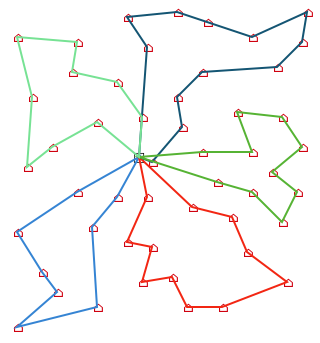
\includegraphics[height=6.5cm]{ui-sample.png}
	\captionof{figure}{Sample of plotting.}
\end{center}

The file generated from the UI is a JSON file with all parameters for the vehicle routing problem and all the $n*n$ distances of each customers.

During the execution of the algorithm, when a new best solution is found it is appended at the end of the file such that is possible to see real time progress. 

%------------------------------------------------

\begin{table*}[ht]
	\caption{Result for \emph{$E$} problem instances}
	\label{tb:res}
	\hspace*{-2cm}\begin{tabular}{l||cccrr||cc|c} 
		\hline
		& & & & & & \multicolumn{2}{c|}{Improvement} \\
		\toprule
		Test & Start Cost & End Cost & Optimal Cost & Overall Time (s) & Best time (m) & Total & \% & \% from optimal \\
		\midrule
		E-n51-k5 & 718 & 521 & 521 & 780 & 4 & 197 & -27.44 & 0.00 \\
		\rowcolor{Gray}
		E-n76-k7 & 869 & 695 & 682 & 16535 & 202 & 174 & -20.02 & 1.91 \\
		E-n76-k8 & 886 & 780 & 735 & 5601 & 26 & 106 & -11.96 & 6,12 \\
		\rowcolor{Gray}
		E-n76-k10 & 1089 & 867 & 830 & 11579 & 143 & 222 & -20.39 & 4,46 \\
		E-n76-k14 & 1176 & 1144 & 1021 & 2881 & 3 & 32 & -2,72 & 12,05 \\
		\rowcolor{Gray}
		E-n101-k8 & 1122 & 887 & 815 & 18817 & 232 & 235 & -20.94 & 8.83 \\
		E-n101-k14 & 1375 & 1197 & 1067 & 18156 & 25 & 178 & -12.95 & 12.18 \\
		\bottomrule
	\end{tabular}
\end{table*}

\section{Results}
The algorithm is implemented in C++ (with support for C++14) and compiled with the GNU Compiler Collection (v.5.3.0) with some optimization, security flags and the \textit{pthread} header for parallel execution.
In addition is embedded a JSON library (rapidjson: \url{https://github.com/miloyip/rapidjson}) for loading and saving data, and the library for parallel execution (ThreadPool: \url{https://github.com/edoz90/threadpool}).\newline
All tests were performed with no verbose flag on a i7-3632QM CPU with 4 core at 3.20GHz and 8 threads.

Routines execution times are measured with the C++ \textit{chrono} library.\newline
Table [\ref{tb:res}] shows the results of some executions on standard data from \url{http://www.coin-or.org/} library.

%------------------------------------------------

\section{Discussion}
This algorithm is only partially parallel and in order to gain the maximum from multi-core CPUs it should run every routine in parallel. 

Future improvement will change the routine of tabu search to make it run on multiple core without losing information and improving the solution quickly.\newline
As the results in table [\ref{tb:res}] show, the algorithm does not find all optimal routes but the solutions found are quite acceptable for this implementation. 

The plotting of non-optimal routes found is good: there is no route that cross over itself or over other routes and the flower pattern is quite respected.\newline
The algorithm with little improvements on logic and parameters value and with more computational power (or execution time) could find a solution with 2-4\% of difference from optimal.

%----------------------------------------------------------------------------------------
%	REFERENCE LIST
%----------------------------------------------------------------------------------------

\begin{thebibliography}{5} % Bibliography - this is intentionally simple in this template

\bibitem[G. Laporte, 2001]{Laporte:2001}
Palgrave Macmillan Journals, J-F Cordeau and G. Laporte and A. Mercier (2001).
\newblock The Journal of the Operational Research Society, vol. 52 (2001).
\newblock {\em A Unified Tabu Search Heuristic for Vehicle Routing Problems with Time Windows}.

\bibitem[Jean-François Cordeau, 2012]{Cordeau:2012}
Elsevier, Jean-François Cordeau, Mirko Mischberger (2001).
\newblock Computers \& Operations Research.
\newblock {\em A parallel iterated tabu search heuristic for vehicle routing problems}.

\bibitem[Michel Gendreau, 1994]{Gendreau:1994}
INFORMS, Michel Gendreau, Alain Hertz, Gilber Laporte (1994).
\newblock Management Science, vol. 40 (1994)
\newblock {\em A Tabu Search Heuristic for the Vehicle Routing Problem}.

\bibitem[Wikipedia, 2016]{Wikipedia:TabuSearch}
Wikipedia, The Free Encyclopedia, Tabu Search (2016).
\newblock \url{https://en.wikipedia.org/wiki/Tabu_search}

\bibitem[Wikipedia, 2016]{Wikipedia:VRP}
Wikipedia, The Free Encyclopedia, Vechicle Routing Problem (2016).
\newblock \url{https://en.wikipedia.org/wiki/Vehicle_routing_problem}

\end{thebibliography}

%----------------------------------------------------------------------------------------

\end{multicols}

\end{document}
